\documentclass{BeamerTemplate}

\title{Module 1 - Introduction aux probabilités}

\subtitle{STT-1900 Méthodes statistiques pour l'ingénierie}
\date{\today}

\begin{document}
\begin{frame}[t]
  \titlepage
\end{frame}

%-------------------------------------------------------------------------------------------------------------------------------------





%%%%%%%%%%%%%%%%%%%%%%%%%%%%%%%%%%%
%%%%%%%%%%%%%%%%%%%%%%%%%%%%%%%%%%%
%%%%%%%%%%%%%%%%%%%%%%%%%%%%%%%%%%%


\section[Statistique]{Importance de  la statistique}

\subsection*{ }

\begin{frame}[t]{Pourquoi un cours de statistique?}
%En génie et en sciences appliquées, on doit souvent concevoir ou analyser des systèmes ou phénomènes dont toutes les caractéristiques ne sont pas \alert{déterministes}, mais plut\^ot \alert{aléatoires}.

Conception ou analyse de systèmes ou phénomènes  \alert{aléatoires}, i.e. non déterministes.

\bigskip
{\ }

 \underline{Exemples:}

\begin{itemize}
\item fiabilité d'une machine industrielle
\item quantité de pluie reçue dans un bassin versant
\item demande en électricité d'un grand édifice à bureaux
%\item durée des périodes sans emploi
\item nombre de tomates produites par un plant
\end{itemize}

\end{frame}

\begin{frame}[t]%{Les probabilités}
 \begin{Boite}{Probabilités}
 Outil mathématique formel  servant à décrire et modéliser les comportements aléatoires.
 \end{Boite}

 \medskip


 \uncover<2->{ \underline{Exemple:} \\Description mathématique du
 comportement d'un dé régulier à 6 faces:
 \begin{itemize}
\item  l'ensemble des résultats possibles est $S=\{1,2,3,4,5,6\}$,
\item la probabilité d'obtenir chacun de ces  résultats lors d'un lancer est 1/6.
\end{itemize}}
\end{frame}

\begin{frame}[t]%{La statistique}
 \begin{Boite}{La statistique}
 Étude  quantitative des attributs d'une «population» à partir  d'observations.
 \end{Boite}

 \medskip
 {\ }

 \uncover<2->{
 $\Rightarrow$ Le caractère \alert{incertain} (non déterministe,
 aléatoire) qui découle de l'échantillonnage des observations fait que la
 statistique est basée sur la théorie des
 probabilités.

 \underline{Exemple:}

 \begin{itemize}
     \item Nous aimerions savoir si un dé à 6 faces est équilibré.
 \end{itemize}
 
 }
\end{frame}
\begin{frame}[t]%{Exemples}

\underline{Exemples de décisions basées sur la statistique:}

 \begin{itemize}
  \item  Sept véhicules d'un même modèle d'une même   année sont impliqués dans des incidents similaires en trois mois. $\Rightarrow$ Doit-on procéder à   un rappel?
  \item  Un futur ponceau doit pouvoir résister à une crue de 100 ans (i.e. dont la probabilité de survenir ou être excédée est de $\frac{1}{100}$ chaque année).
  \item  Trois types d'apprêt   peuvent être appliqués à des échantillons   d'aluminium  à l'aide de  deux méthodes différentes. Y a-t-il une   combinaison apprêt-méthode  qui se démarque?
 \end{itemize}
 \uncover<2->{
  $\Rightarrow$ Une bonne compréhension des probabilités et de la
  statistique est \alert{indispensable} à la prise de décision
  en présence d'incertitude!
 }
\end{frame}


\section[Expérience aléatoire]{Expérience aléatoire et espace échantillonnal}

%\subsection{Définitions et notation}

\begin{frame}[t]%{Expérience aléatoire, espace échantillonnal}

 \begin{Boite}{Expérience aléatoire $\cal{E}$}
Expérience dont le résultat dépend du hasard, ne pouvant  être prédit avec certitude.
\end{Boite}

 \begin{Boite}{Espace échantillonnal $S$}
Ensemble de tous les résultats possibles de l'expérience ${\cal{E}}$.
\end{Boite}


 \medskip
\begin{itemize}
\item \alert{$S$ discret}:
 Si $S$ est dénombrable (peut être fini ou infini) \\(ex: la liste des entiers)

\item \alert{$S$ continu}:
 Si $S$ est  non dénombrable \\(ex: un intervalle de valeurs sur la droite réelle)
 \end{itemize}


\end{frame}

\begin{frame}[t]{Exemple 1: Quel est l'espace échantillonnal?}

 \begin{itemize}\itemsep 10mm
  \item<1-> ${\cal{E}}_1$: On roule un dé ordinaire et on note le chiffre sur la
  face du dessus.% \uncover<2->{\alert{ $\Rightarrow {{S}}_1=\{1,2,3,4,5,6\}$.}}
  \item<1-> ${\cal{E}}_2$: On pige une carte parmi les quatre rois d'un jeu standard.
  %\uncover<2-> {\alert{$\Rightarrow {{S}}_2=\{R\spadesuit,R\heartsuit,R\diamondsuit,R\clubsuit\}$.}}
  \item<1-> ${\cal{E}}_3$: On compte le nombre de véhicules traversant un pont durant
  une heure. %\uncover<2->{\alert{ $\Rightarrow {{S}}_3=\{0,1,2,\ldots\}$.}}
  \item<1-> ${\cal{E}}_4$: On mesure la quantité de pluie (en mm) reçue à une station
  météo au cours de l'automne. %\uncover<2->{\alert{ $\Rightarrow {{S}}_4=\{x:x\ge0\}$.}}
 \end{itemize}
\end{frame}

\subsection{Événements}

\begin{frame}[t]%{Définition et exemples}
 \begin{Boite}{Événement}
  Sous-ensemble de l'espace   échantillonnal $S$. \\On utilise  une lettre majuscule pour l'identifier. %[Si ${{S}}$ est un ensemble   fini, alors l'ensemble de tous les événements possibles   est l'ensemble puissance $\{0,1\}^{{{S}}}$.]
 \end{Boite}

 \medskip

 \uncover<2->{ Retour aux 4 expériences aléatoires, exemples d'événements:
 \small
  \begin{itemize}\itemsep 5mm
   \item ${\cal{E}}_1$: \alert{$A$}=«Le dé affiche un nombre pair»=$\{2,4,6\}$
   \item ${\cal{E}}_2$: \alert{$N$}=«On pige un roi noir»=$\{R\spadesuit,R\clubsuit\}$
   \item ${\cal{E}}_3$: \alert{$C$}=«Moins de 100 véhicules traversent le pont» =$\{0,1,2,\ldots,99\}$
   \item ${\cal{E}}_4$: \alert{$D$}=«La station reçoit plus de 150 mm de pluie»=$(150,\infty)$
  \end{itemize}
 }
\end{frame}


\begin{frame}{Rappel des opérations sur les ensembles}
\begin{columns}
\column{0.5\textwidth}
\textbf{1) Complément de A : $\overline{A}$}
\vspace{0.2cm}

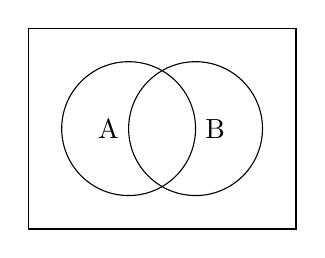
\begin{tikzpicture}[scale=0.85]
  \draw (0,0) rectangle (4,3);
  % \begin{scope}
  % \fill[gray!30] (0,0) rectangle (4,3);
  %   \clip (0,0) rectangle (4,3);
  %   \fill[gray!30] (2.5,1.5) circle (1);
  %   \fill[white] (1.5,1.5) circle (1);
  % \end{scope}
  \draw (1.5,1.5) circle (1) node[left] {A};
  \draw (2.5,1.5) circle (1) node[right] {B};
\end{tikzpicture}

\vspace{0.4cm}
\textbf{3) Intersection de A et B : $A \cap B$}
\vspace{0.2cm}

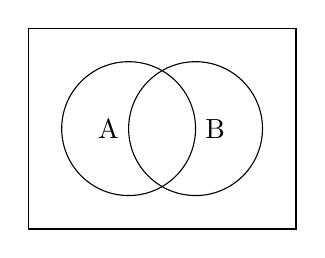
\begin{tikzpicture}[scale=0.85]
  \draw (0,0) rectangle (4,3);
  % \begin{scope}
  %   \clip (1.5,1.5) circle (1);
  %   \fill[gray!30] (2.5,1.5) circle (1);
  % \end{scope}
  \draw (1.5,1.5) circle (1) node[left] {A};
  \draw (2.5,1.5) circle (1) node[right] {B};
\end{tikzpicture}

\column{0.5\textwidth}
\textbf{2) Inclusion de B dans A : $B \subset A$}
\vspace{0.2cm}

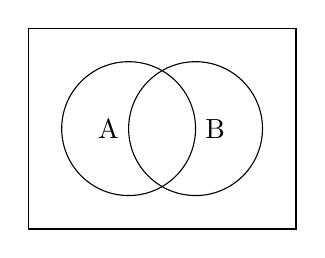
\begin{tikzpicture}[scale=0.85]
  \draw (0,0) rectangle (4,3);
  % \begin{scope}
  %   \clip (1.5,1.5) circle (1);
  %   \fill[gray!30] (2.5,1.5) circle (1);
  % \end{scope}
  \draw (1.5,1.5) circle (1) node[left] {A};
  \draw (2.5,1.5) circle (1) node[right] {B};
\end{tikzpicture}
% \begin{tikzpicture}[scale=0.85]
%  \draw (0,0) rectangle (5,3);
%   \draw (2.5,1.5) circle (1.2);
%   \node at (1.6,1.8) {A};
%   \draw (2.5,1.5) circle (0.6);
%   \node at (2.5,1.5) {B};
% \end{tikzpicture}

\vspace{0.4cm}
\textbf{4) Union de A et B : $A \cup B$}
\vspace{0.2cm}

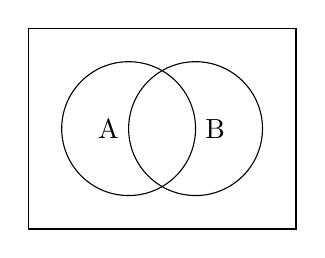
\begin{tikzpicture}[scale=0.85]
  \draw (0,0) rectangle (4,3);
  % \begin{scope}
  %   \clip (0,0) rectangle (4,3);
  %   \fill[gray!30] (1.5,1.5) circle (1);
  %   \fill[gray!30] (2.5,1.5) circle (1);
  % \end{scope}
  \draw (1.5,1.5) circle (1) node[left] {A};
  \draw (2.5,1.5) circle (1) node[right] {B};
\end{tikzpicture}
\end{columns}
\end{frame}


\begin{frame}{Rappel des opérations sur les ensembles}
\begin{columns}
\column{0.5\textwidth}
\textbf{1) Complément de A : $\overline{A}$}
\vspace{0.2cm}

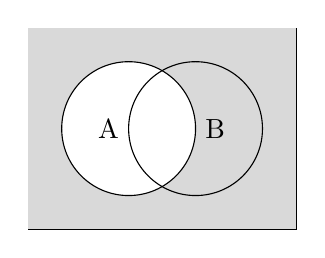
\begin{tikzpicture}[scale=0.85]
  \draw (0,0) rectangle (4,3);
  \begin{scope}
  \fill[gray!30] (0,0) rectangle (4,3);
    \clip (0,0) rectangle (4,3);
    \fill[gray!30] (2.5,1.5) circle (1);
    \fill[white] (1.5,1.5) circle (1);
  \end{scope}
  \draw (1.5,1.5) circle (1) node[left] {A};
  \draw (2.5,1.5) circle (1) node[right] {B};
\end{tikzpicture}

\vspace{0.4cm}
\textbf{3) Intersection de A et B : $A \cap B$}
\vspace{0.2cm}

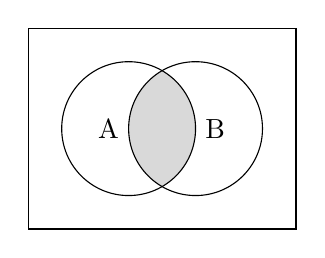
\begin{tikzpicture}[scale=0.85]
  \draw (0,0) rectangle (4,3);
  \begin{scope}
    \clip (1.5,1.5) circle (1);
    \fill[gray!30] (2.5,1.5) circle (1);
  \end{scope}
  \draw (1.5,1.5) circle (1) node[left] {A};
  \draw (2.5,1.5) circle (1) node[right] {B};
\end{tikzpicture}

\column{0.5\textwidth}
\textbf{2) Inclusion de B dans A : $B \subset A$}
\vspace{0.2cm}

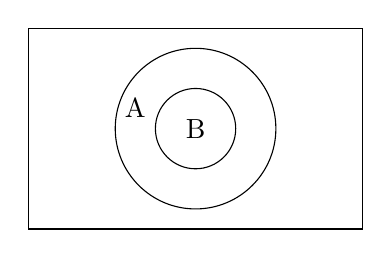
\begin{tikzpicture}[scale=0.85]
 \draw (0,0) rectangle (5,3);
  \draw (2.5,1.5) circle (1.2);
  \node at (1.6,1.8) {A};
  \draw (2.5,1.5) circle (0.6);
  \node at (2.5,1.5) {B};
\end{tikzpicture}

\vspace{0.4cm}
\textbf{4) Union de A et B : $A \cup B$}
\vspace{0.2cm}

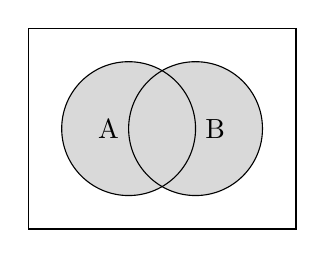
\begin{tikzpicture}[scale=0.85]
  \draw (0,0) rectangle (4,3);
  \begin{scope}
    \clip (0,0) rectangle (4,3);
    \fill[gray!30] (1.5,1.5) circle (1);
    \fill[gray!30] (2.5,1.5) circle (1);
  \end{scope}
  \draw (1.5,1.5) circle (1) node[left] {A};
  \draw (2.5,1.5) circle (1) node[right] {B};
\end{tikzpicture}
\end{columns}
\end{frame}

\begin{frame}[t]%{Événements mutuellement exclusifs}
 \begin{Boite}{Événements mutuellement exclusifs}
  Des événements sont \alert{mutuellement exclusifs} si toutes
  leurs combinaisons possibles d'intersections sont vides, c'est-à-dire
  lorsqu'\textbf{au plus un} de ces événements peut se produire à
  la fois. %On dit aussi que ces événements sont \alert{incompatibles} ou \alert{disjoints}.
 \end{Boite}

 \medskip


 {\small \uncover<2->{ %Retour aux exemples:

 En d'autres termes, $A$, $B$ et $C$ sont mutuellement exclusifs, si

  \begin{itemize}
   \item $A\cap B=\emptyset$
   \item $A\cap C=\emptyset$
   \item $B\cap C=\emptyset$
   \item $A\cap B\cap C=\emptyset$
 \end{itemize}
 }}
\end{frame}


\begin{frame}[t]%{Événements mutuellement exclusifs}

\centerline{\LARGE \bf \alert{QUIZ !}}

 Les événements suivants sont-ils mutuellement exclusifs?
 \medskip

 {\small  %Retour aux exemples:
  \begin{itemize}\itemsep1.3cm
   \item ${\cal{E}}_1$: Lancer d'un dé.\\
   Soit $A=$«obtenir un nombre pair», $B=\{5\}$ et $C=\{1\}$. \\
   %Comme    $A\cap B=A\cap C=B\cap C=A\cap B\cap C=\emptyset$, ces trois    événements sont mutuellement exclusifs.
   \item<2-> ${\cal{E}}_4$: Mesurer les précipitations.\\
   $A=$«La station reçoit plus de 150 mm»,\\
   $B=$«La station reçoit moins de 175 mm» et \\$C=$«La station reçoit
   entre 200 et 300 mm». \\%Comme $A\cap B=(150,175)\neq\emptyset$,     $A,B,C$ ne sont \alert{pas} mutuellement exclusifs. (Même si $B$ et $C$ le sont.)
   %(On aurait aussi pu    utiliser $A\cap C=(300,\infty)\neq\emptyset\ldots$)
   \vspace{1.3cm}
 \end{itemize}
 }
\end{frame}



%\section{Dénombrement des espaces échantillonnaux finis}
%
%\subsection{Nombre de sous-ensembles}
%
%\begin{frame}[t]{Taille de l'ensemble-puissance}
%Dans plusieurs applications, il faudra conna\^{\i}tre le nombre
%d'éléments formant un événement afin d'en calculer la
%probabilité. Plusieurs règles de calcul reviennent souvent.
%
%\medskip
%\uncover<2->{
% \begin{Boite}{Nombre de sous-ensembles}
%  Soit $A$ un ensemble contenant $m$ éléments (i.e., $n(A)=m$).
%  Alors l'ensemble puissance de $A$ compte $2^m$ éléments
%  (i.e., $n\left(\{0,1\}^A\right)=2^m$).
% \end{Boite}}
%
%\medskip
%\uncover<3->{ Soit $B=\{1,2,3\}$. On a vu plus t\^ot que $\{0,1\}^B$ comptait
% $8=2^3$ éléments.}
%\end{frame}
%
%\subsection{Diagrammes}
%
%\begin{frame}[t]{Diagrammes en arbre}
%Dans plusieurs problèmes, lorsque le nombre d'éléments à dénombrer
%n'est pas trop grand, on peut \alert{lister explicitement} tous les éléments
%de l'espace échantillonnal et compter combien forment l'événement d'intérêt.
%
%\medskip
%
%Souvent, pour n'oublier aucune possibilité, on s'aide d'un schéma, comme par
%exemple en faisant un diagramme en arbre.
%\end{frame}
%
%\begin{frame}[t]{Exemple de diagramme en arbre}
%Soit l'expérience o\`u l'on tire un pièce de monnaie et ensuite on roule
%un dé régulier. Combien y a-t-il d'éléments dans l'espace échantillonnal?
%De combiens d'éléments sont formés les événements
%$A=$«le dé indique un nombre pair» et $B=$«la pièce indique face et le
%dé indique un nombre impair»?
%\end{frame}
%
%\subsection{Principe de multiplication}
%
%\begin{frame}[t]{Le principe}
%
% \begin{Boite}{Principe de multiplication}
%  Si les ensembles $A_1,A_2,\ldots,A_k$ comptent respectivement
%  $n_1,n_2,\ldots,n_k$ éléments, alors il existe $n_1n_2\cdots n_k$
%  façons de choisir un élément de $A_1$, un élément de $A_2$,
%  $\ldots$, un élément de $A_k$.
% \end{Boite}
%
% \medskip
%
% \uncover<2->{
% \underline{Exemple}: Un code postal est composé d'une lettre, un chiffre,
% un lettre, un chiffre, une lettre et un chiffre. On a donc en principe
% $26\times10\times26\times10\times26\times10=17~576~000$ possibilités
% de code postaux.
% }
%\end{frame}
%
%\begin{frame}[t]{Expériences aléatoires composées}
%Une conséquence utile du principe de multiplication est
%que si une expérience aléatoire ${\cal{E}}$ est composée d'une
%suite de $k$ expériences aléatoires
%${\cal{E}}_1$, ${\cal{E}}_2$, $\ldots$, ${\cal{E}}_k$ ayant pour
%espaces échantillonnaux respectifs $S_1,S_2,\ldots,S_k$ avec
%$n(S_1)=n_1$, $n(S_2)=n_2$, $\ldots$, $n(S_k)=n_k$, alors
%le nombre de résultats possibles de ${\cal{E}}$ est
%$n_1n_2\cdots n_k$.
%
%\medskip
%
% \uncover<2->{
%  Dans l'exemple de la pièce de monnaie et du dé, on pouvait voir
%  ${\cal{E}}$ comme une suite de deux expériences ${\cal{E}}_1$ et
%  ${\cal{E}}_2$ avec $S_1=\{P,F\}$, $S_2=\{1,2,3,4,5,6\}\Rightarrow n_1=2$,
%  $n_2=6$ et $n_1n_2=2\times6=12$.
% }
%\end{frame}
%
%\subsection{Permutations}
%
%\begin{frame}[t]{Définition et un exemple}
% \begin{Boite}{Définition}
%  Une \alert{permutation} est un arrangement \alert{ordonné}
%  d'objets \alert{distincts}.
% \end{Boite}
%
% \medskip
%
% \uncover<2->{
%  \underline{Exemple}: Supposons 3 fusibles: un de 10 ampères, un de 15 ampères
%  et un de 20 ampères. Soit les circuits 1 et 2. De combien de façons
%  différentes peut-on assigner les 3 fusibles aux 2 circuits?
% }
%
% \vspace{1in}
%
% {\small\uncover<3->{$\Rightarrow$ On a 6 \alert{permutations} possibles
% de 3 objets pris deux à la fois.}}
%\end{frame}
%
%\begin{frame}[t]{Formule générale}
%
% \begin{Boite}{Nombre de permutations possibles}
%  Le nombre de permutations possibles de $n$ objets pris $r$
%  à la fois est donné par
%  $$P_r^n=n(n-1)\cdots(n-r+1)=\frac{n!}{(n-r)!}.$$
% \end{Boite}
%
% \medskip
%
% \uncover<2->{
%  Ce résultat vient du \alert{principe de multiplication}: nous avons $n$
%  choix d'objets pour la première position, $n-1$ choix d'objets pour la
%  seconde position, ..., $n-r+1$ choix d'objets pour la $r$-ème position.
% }
%
% \medskip
%
% \uncover<3->{ [Rappel: $n!=n(n-1)(n-2)\cdots1$; $0!=1!=1$; donc $P_n^n=n!$.]}
%\end{frame}
%
%\begin{frame}[t]{Exemple}
% Dix pilotes sont disponibles pour assurer quatre liaisons aériennes. Combien
% d'options d'assignation de ces pilotes à ces liaisons a-t-on?
%
% \medskip
%
% \uncover<2->{
%  $P^{10}_4=\frac{10!}{(10-4)!}=\frac{10!}{6!}=
%  \frac{10\times9\times\cdots\times1}{6\times5\times\cdots\times1}=10\times9\times8\times7=5~040$.
% }
%
% \bigskip
%
% \uncover<3->{
%  Pour les mêmes 4 liaisons aériennes, on doit choisir 4 équipages de bord parmi
%  12 équipages disponibles. De combien de façons différentes peut-on
%  assigner les pilotes ET les équipages de bord aux 4 liaisons?}
%
%  \medskip
%
%  {\small \uncover<4->{
%   Pour les équipages de bord: $P^{12}_4=12\times11\times10\times9=11~880$.\\
%   {\ }\\
%   De la règle de multiplication, on a $5~040\times11~880=59~875~200$ façons
%   d'assigner les pilotes et les équipages de bord aux 4 liaisons.
%  }
% }
%\end{frame}
%
%\section{Combinaisons}
%
%\begin{frame}[t]{Définition et un exemple}
% \begin{Boite}{Définition}
%  Une \alert{combinaison} est un arrangement
%  \alert{non ordonné} d'objets \alert{distincts}.
% \end{Boite}
%
% \medskip
%
% \uncover<2->{
%  Je dois choisir 2 de mes 3 meilleurs amis pour aller dans le Sud avec
%  moi. Combien d'options ais-je?
% }
%
% \medskip
%
% \uncover<3->{
%  Soit $a,b,c$, mes trois meilleurs amis. J'aurais $P^3_2=6$ permutations de
%  ces 3 amis pris 2 à la fois ... mais je compterais $(a,b)$ et $(b,a)$ deux fois
%  alors qu'il s'agit d'une seule et même option!\\
%  En fait de dois diviser
%  $P^3_2$ par 2 pour obtenir 3 choix possibles, Soit
%  $(a,b)$, $(a,c)$ ou $(b,c)$.
% }
%\end{frame}
%
%\begin{frame}[t]{Formule générale}
% \begin{Boite}{Nombre de combinaisons}
%  Le nombre de combinaisons possibles de $r$ objets pris parmi $n$ est
%  $${n\choose r}=C^n_r=\frac{n!}{r!(n-r)!}.$$
% \end{Boite}
%
% \medskip
%
% \uncover<2->{
%  On peut utiliser la règle de multiplication et le nombre de permutations
%  de $n$ objets pris $r$ à la fois pour voir d'o\`u vient cette formule.\\
%
%  Soit $x$, le nombre de façons de choisir $r$ objets parmi $n$. Alors on
%  a que $P^n_r=x\times P^r_r=x\times r!$, car une permutation consiste tout
%  d'abord à choisir $r$ objets parmi les $n$, ensuite à permuter ces
%  $r$ objets.
%
%  Donc $P^n_r=xr! \Rightarrow x=P^n_r/r!=\frac{n!}{(n-r)!}\frac{1}{r!}=
%  \frac{n!}{r!(n-r)!}$.
% }
%\end{frame}
%
%\begin{frame}[t]{Exemples}
% \begin{itemize}
%  \item<1->{\bf Lotto 6/49}: On tire au hasard 6 des 49 nombres de 1 à 49, et l'ordre dans
%  lequel les 6 nombres sont tirés ne compte pas. On a donc
%  \uncover<2->{
%  $${49\choose6}=\frac{49!}{6!43!}=\frac{49\times48\times47\times46\times45\times44}{6!}=
%  13~983~816$$
%  combinaisons possibles. On aurait pu trouver aussi à l'aide de la règle de multiplication:
%  49 choix pour le 1er nombre, 48 pour le second, ... 44 pour le 6e, et ensuite on doit diviser
%  par $6!$ car chaque combinaison est comptée $6!$ fois.}
% \end{itemize}
%\end{frame}
%
%\begin{frame}[t]{Exemples}
% \begin{itemize}
%  \item<1->{\bf Poker}: Au poker, une main consiste en 5 cartes tirées d'un jeu de 52 cartes
%  distinctes. Il y a donc \uncover<2->{
%  $${52\choose5}=\frac{52!}{5!47!}=\frac{52\times51\times50\times49\times48}{5!}=
%  2~598~960$$
%  mains de poker distinctes.}
%  \item<3->{\bf Paires}: Des 2~598~960 mains de poker possibles, combien se qualifient
%  de «une paire»?
% \end{itemize}
%\end{frame}
%
%\begin{frame}[t]{Exemples (suite)}
% \begin{itemize}
%  \item<1->{\bf Comités:} Un groupe de 30 personnes doit choisir 4 représentants. Combien y a-t-il
%  de comités possibles? Et si le comité est formé d'un président, d'un V-P, d'un trésorier,
%  et d'un secrétaire? Et si le comité est formé d'un président et de 3 autres membres?
% \end{itemize}
%\end{frame}
%
%\begin{frame}[t]{Propriétés importante}
%
% \begin{Boite}{Théorème du bin\^ome}
%  Soit deux nombres réels $x$ et $y$ et un entier $n$. Alors
%  $$(x+y)^n=\sum_{r=0}^n{n\choose r}x^ry^{n-r}.$$
% \end{Boite}
%
% \medskip
%
% \uncover<2->{
% \begin{Boite}{Échantillonage}
%  Le nombre de combinaisons ${n\choose r}$ représente aussi
%  le nombre d'échantillons différents qui peuvent
%  être obtenus lorsque l'on tire \alert{sans remise} $r$ objets
%  d'une population de $n$ objets distincts.
% \end{Boite}
% }
%\end{frame}
%
%\begin{frame}[t]{Identités}
% \begin{itemize}
%  \item<1-> ${n\choose r}={n\choose n-r}$
%  \item<2-> ${n\choose r}={n-1\choose r-1}+{n-1\choose r}$
%  \item<3-> $2^n=(1+1)^n=\sum_{r=0}^n {n\choose r}1^r1^{n-r}={n\choose0}+{n\choose1}
%  +\cdots+{n\choose n}$
% \end{itemize}
%\end{frame}
%

\section{Probabilités}

\subsection{Définitions et notation}

\begin{frame}[t]%{Définition mathématique}

{\small  \begin{Boite}{Probabilité: Définition axiomatique}
  Soit une expérience aléatoire ${\cal{E}}$, son espace échantillonnal $S$ et un événement $A$ défini dans $S$. \\
  La \alert{probabilité d'un événement, notée $P(\centerdot)$}, est un nombre réel respectant les axiomes
  suivants:
  \begin{enumerate}
   \item $0\le P(A)\le 1$
   \item $P(S)=1$
   \item Pour toute suite d'événements \alert{mutuellement exclusifs}
   $A_1,A_2,\ldots,A_k$ définis dans $S$, on a
   $$P(A_1\cup A_2\cup \cdots \cup A_k)=P(A_1)+P(A_2)+\cdots+P(A_k)$$
   \item L'axiome 3 reste vrai quand $k\to\infty$ :\ $P\left(\bigcup_{i=1}\limits^\infty A_i\right)=\sum\limits_{i=1}^\infty P(A_i)$.
  \end{enumerate}
 \end{Boite}
}
\end{frame}

\begin{comment}
\begin{frame}[t]{Spécification des probabilités}
Comment peut-on déterminer des probabilités?
\medskip

 \begin{itemize}\itemsep8mm
  \item<1-> estimations basées sur des observations
  \item<2-> analyse des conditions expérimentales
  \item<3-> modèles probabilistes et/ou hypothèses
 \end{itemize}
\end{frame}


\begin{frame}[t]{Interprétation en termes de fréquences }
 Intuitivement, on peut voir la probabilité d'un événement $A$
 comme la \alert{proportion des fois o\`u il surviendrait} si on
 répétait la même expérience un très grand nombre de fois.

 \medskip
 \uncover<2->{
  \begin{Boite}{Fréquence relative d'un événement}
   On répète $m$ fois une expérience ${\cal{E}}$.\\
   Soit $m_A$ le nombre de fois o\`u l'événement $A$ se produit.
   Alors    $$f_A=\frac{m_A}{m}$$ est la \alert{fréquence relative} de l'événement $A$.
  \end{Boite}
 }
\end{frame}

\begin{frame}[t]{Propriétés des fréquences relatives}
 \begin{enumerate}
  \item $0\le f_A\le 1$
  \item $f_A=0\Leftrightarrow$ $A$ ne se produit jamais, et\\
  $f_A=1\Leftrightarrow A$ se produit à tout coup
  \item Si $A$ et $B$ sont mutuellement exclusifs,
  alors $f_{A\cup B}=f_A+f_B$
 \end{enumerate}

 \medskip
 \uncover<2-> {
  Très près des axiomes qui définissent $P(A)$ ...

  \bigskip
  En fait comme $f_A$ tend à se stabiliser quand $m$ devient très
  grand, on pourrait définir $P(A)=\lim\limits_{m\to\infty} \dfrac{m_A}{m}$.
 }
\end{frame}

%\begin{frame}[t]{Cas équiprobable}
%
% Supposons que $S$ est constitué d'un nombre $n$ fini d'éléments,
% $S=\{e_1,e_2,\ldots,e_n\}$. Supposons aussi que la probabilité attribuée
% à chacun de ces éléments est la même, i.e., si $E_i=$«le résultat
% $e_i$ se produit», alors $p_i=P(E_i)=1/n$ pour tout $i=1,\ldots,n$.
%(On dit dans ce cas
% que les éléments de $S$ sont \alert{équiprobables}.)
%
%  \bigskip
%
% {\ }
%
% Dans ce cas équiprobable, nous pouvons calculer la probabilité de tout événement $A$
% en dénombrant ses éléments. En effet, puisque les $e_i$ sont mutuellement
% exclusifs et que $A$ est une union de $e_i$, on a de l'axiome 3
% $$P(A)=P\left(\bigcup_{i:e_i\in A}e_i\right)=\sum_{i:e_i\in A}P(e_i)=
% \sum_{i:e_i\in A}1/n=\frac{n(A)}{n}.$$
%\end{frame}
%
%\begin{frame}[t]{Retour aux exemples}
% \begin{itemize}
%  \item<1-> Vous achetez un billet avec 5 combinaisons distinctes pour le
%  prochain tirage du Lotto 6/49. Quelle est votre probabilité de
%  gagner le prochain gros lot?
%
%  \uncover<2->{
%   Comme on l'a vu, on a un espace échantillonnal fini constitué
%   de 13~983~816 éléments ($n=13~983~816$). L'événement $A=$«vous gagnez le gros lot»
%   est constitué de 5 éléments ($n(A)=5$). Donc $P(A)=5/13~983~816\approx 0.00000036$.
%  }
%
%  \item<3-> Vous pigez 5 cartes. Quelle est la probabilité que vous ayez la main
%  de poker «une paire»?
%
%  \uncover<4->{
%   On a vu qu'il y a $2~598~960$ mains possibles. Si le brasseur ne triche pas,
%   ces mains devraient être équiprobables. Soit $B=$«avoir une paire». Comme
%   $n(B)=1~098~240$, on a que $P(B)=1~098~240/2~598~960=352/833\approx0.42$.
%  }
% \end{itemize}
%\end{frame}
\end{comment}


\subsection{Propriétés}

\begin{frame}[t]{Résultats découlant des axiomes}
Les résultats qui suivent sont des conséquences des 4 axiomes
définissant une probabilité. 

 \begin{itemize}
  \item<1->{\bf Théorème 1.1}: $P(\emptyset)=0$

  {\color{gray}{[$S$ et $\emptyset$ sont mutuellement
  exclusifs, $S\cup\emptyset=S$ et $P(S)=1$ ...]}}
  \item<2->{\bf Théorème 1.2}: $P(\bar{A})=1-P(A)$

  {\color{gray}{[$A$ et $\bar{A}$ sont mutuellement
  exclusifs et $S=A\cup\bar{A}$ ...]}}
  \item<3->{\bf Théorème 1.3}: $P(A\cup B)=P(A)+P(B)-P(A\cap B)$

  \item<4->{\bf Théorème 1.4}:
  $$\begin{array}{lll}
  P(A\cup B\cup C)&=&P(A)+P(B)+P(C)\\&&-P(A\cap B)
   -P(A\cap C)-P(B\cap C)\\&&+P(A\cap B\cap C)\end{array}$$

  % [Un peu long, mais se démontre en appliquant le théorème 1.3 à $D\cup C$, o\`u    $D=A\cup B$, et en réalisant que $A\cup B\cup C=D\cup C$ ...]
 \end{itemize}
\end{frame}

\begin{frame}[t]{Résultats découlant des axiomes (suite)}
 \begin{itemize}\itemsep6mm
  \item<1->{\bf Théorème 1.5}: Généralisation de 1.4 à $k$ événements:
     \\
$P\left(\bigcup\limits_{i=1}^kA_i\right)=\sum\limits_{i=1}^kP(A_i)
  -\sum\limits_{i=1}^k\sum\limits_{j=i+1}^kP(A_i\cap A_j)+\cdots+(-1)^{k-1}P\left(\bigcap\limits_{i=1}^kA_i\right)$

  \item<2->{\bf Théorème 1.6}: Si $A\subset B$, alors $P(A)\le P(B)$.

  {\small \color{gray}{[$B=(\bar{A}\cap B)\cup A$, et $(\bar{A}\cap B)$ et $A$ sont mutuellement exclusifs ...]}}
 \end{itemize}
\end{frame}

\begin{frame}[t]{Résultats utiles}
    Ces deux résultats peuvent être utiles:
    \begin{align*}
        P(\overline{A\cap B}) &= P(\overline{A} \cup \overline{B})\\
        P(\overline{A\cup B}) &= P(\overline{A} \cap \overline{B})
    \end{align*}
\end{frame}
\begin{frame}[t]{Exemple 2}

\begin{minipage}{8cm}{
\small
Vous achetez un nouveau téléphone. \\
Définissons les événements suivants:\\
$A$: La carte SIM est défectueuse.\\
$B$: La batterie a une autonomie insuffisante.\\
}
\end{minipage}

\vspace{.3cm}

Chez ce fournisseur, $P(A)=0,05$, $P(B)=0,20$ et $P(A \cup B)=0,23$.

\begin{enumerate}[{a)}]\itemsep1cm
  \item Quelle est la probabilité que votre batterie dure suffisamment longtemps?
  \item Quelle est la probabilité que les deux problèmes Soit présents sur le téléphone que vous avez acheté?
\end{enumerate}
\end{frame}
\begin{frame}[plain,t]


\centerline{\LARGE\bf \alert{ QUIZ! }}

Dans l'exemple précédent, quelle est la probabilité qu'aucun des deux problèmes n'affecte votre téléphone?

 \bigskip



 \bigskip
Rappel:   $P(A)=0,05$, $P(B)=0,20$ et $P(A \cup B)=0,23$.
\vspace{3cm}

\end{frame}

\begin{comment}
\begin{frame}[t]{Exemple}
\small
 $P(A)=0,05$, $P(B)=0,20$ et $P(A \cup B)=0,23$.

\begin{enumerate}\itemsep 1.4cm
  \item[{c)}] Quelle est la probabilité qu'aucun des deux problèmes n'affecte votre téléphone?
  \item[{d)}] Tracez le diagramme de Venn de ces ensembles en inscrivant les probabilités dans les régions représentées.
\end{enumerate}

\end{frame}
\end{comment}
\begin{frame}[t]{Exemple 3}

\small
 Dans une certaine firme de génie,
 \begin{enumerate}[$\bullet$]
 \item 55\% des employés ont au moins une maîtrise,
 \item 70\% des employés font au moins une journée de télétravail,
 \item 75\% des employés habitent à moins de 30 km de leur lieu de travail principal.
 \end{enumerate}
 

\end{frame}

 \begin{frame}[t]{Exemple 3 (suite)}
 \small{
 Si on choisit un employé au hasard dans cette firme, pouvez-vous déterminer la probabilité qu'il s'agisse...
  \begin{enumerate}[(i)]\itemsep.8cm
 \item d'un employé qui n'a pas de maîtrise? % 0.45

 \end{enumerate}
}
\end{frame}

\begin{frame}[t]{Exemple 3 (suite)}

{\footnotesize
 On vous informe maintenant que dans cette firme,
 \begin{enumerate}[$\bullet$]
 \item 35\%  des employés ont une maîtrise et font du télétravail,
 \item 30\% ont une maîtrise, font du télétravail et habitent à moins de 30 km de leur lieu de travail,
 \item 5\% ont une maîtrise, ne font pas de télétravail et n'habitent pas à moins de 30 km de leur lieu de travail.
%  \item 13\% sont des garçons  satisfaits de leurs études.
 \end{enumerate}
 Pouvez-vous maintenant déterminer la probabilité qu'un employé choisi au hasard...
     \begin{enumerate}\itemsep 5mm
      \item[(ii)] ait une maîtrise et habite à moins de 30 km de son lieu de travail?% 0.45
      \item[(iii)] n'ait pas de lunettes et habite à moins de 30 km de son lieu de travail? %0.30
      \item[(iv)] ait une maîtrise ou habite à moins de 30 km de son lieu de travail?% 0.85
     \end{enumerate}
}
\end{frame}

\begin{frame}[t]{Exemple 3: piste de solution}

{\small
 Remplir toutes les zones mutuellement exclusives d'un diagramme de Venn.\\
 $M=$ <<l'employé a une maîtrise>>, $T=$ <<l'employé fait du télétravail>> et $H=$ <<l'employé habite à moins de 30 km de son lieu de travail>>. %On cherche (i) $P(\bar{F}\cap P\cap \bar{S})$ et (ii) $P(F\cap \bar{P}\cap S)$.
}


\begin{center}
    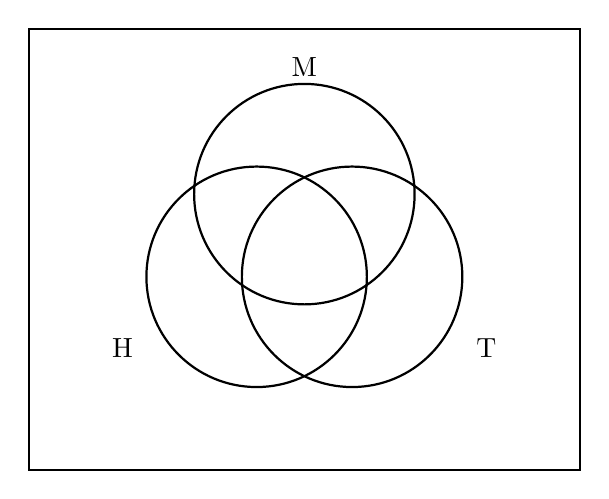
\begin{tikzpicture}[scale = 0.7]
  % Le rectangle
  \draw[thick] (-5,-4) rectangle (5,4);
  
  % Les cercles
  \draw[thick] (-0.866,-0.5) circle (2);     % S
  \draw[thick] (0.866,-0.5) circle (2);      % P
  \draw[thick] (0,1) circle (2);    % F
  
  % Les lettres
  \node at (-3.3,-1.8) {H};
  \node at (3.3,-1.8) {T};
  \node at (0,3.3) {M};
  
\end{tikzpicture}
\end{center}



\end{frame}

\section[Prob. conditionnelles]{Les probabilités conditionnelles}
\begin{frame}[t]{Exemple 3: des infos partielles}
\begin{enumerate}
\item Si on vous disait que l'employé choisi habite à moins de 30 km de son lieu de travail, pourriez-vous déterminer la probabilité qu'il ait une maîtrise?

\vspace{1.3cm}

\item Sauriez-vous déduire de vos informations la probabilité qu'un employé avec une maîtrise choisi au hasard fasse du télétravail?

\vspace{1.3cm}
\end{enumerate}

Pour faire ces calculs, vous devez utiliser une information partielle, qui réduit l'espace échantillonnal. Vous calculerez des {\it probabilités conditionnelles}...

\end{frame}



\subsection{Définition et interprétation}

\begin{comment}
\begin{frame}[t]{Réduction de l'espace échantillonnal}
 \begin{itemize}
  \item<1-> Toutes les probabilités vues jusqu'à maintenant sont  calculées par rapport à l'espace échantillonnal $S$. Nous aurions    pu utiliser une notation du type $P(A|S)$.
  \item Il arrive que nous possédions de l'information partielle   qui élimine la possibilité que certains résultats de l'espace   échantillonnal se produisent. \\$\Rightarrow$ Comment calculer les probabilités   d'événements en présence de telle information?
 \end{itemize}
\end{frame}
\begin{frame}[t]{Exemple illustratif}
 \begin{enumerate}[$\bullet$]\itemsep3mm
 \item On vous dit que 70\% des pièces électroniques que vous utilisez viennent de l'usine A et que les autres pièces viennent de l'usine B.
 \item On vous dit aussi que 25\% de toutes les pièces sont défectueuses.
 \item 10\% de toutes les pièces viennent de l'usine A et sont défectueuses.
 \item[a)] On vous donne une  pièce qui vient de l'usine A. Quelle est la probabilité qu'elle soit défectueuse?
\item[b)] On vous donne une pièce défectueuse. Quelle est la probabilité qu'elle proviennent de l'usine B?
     \end{enumerate}
\end{frame}
\end{comment}

\begin{frame}[t]%{Probabilité conditionnelle}
 \begin{Boite}{Probabilité conditionnelle}
  Soit $A$ et $B$ deux événements dans $S$ avec $P(B)>0$. Alors
  la \alert{probabilité conditionnelle} de $A$  sachant que  $B$ s'est réalisé est
  $$P(A|B)=\frac{P(A\cap B)}{P(B)}.$$
 \end{Boite}
\end{frame}

\begin{frame}[t]{Propriétés}
 %Des 4 axiomes définissant une probabilité et de la définition  d'une probabilité conditionnelle, on peut facilement déduire les propriétés suivantes.



 \begin{enumerate}\itemsep3mm
  \item $0\le P(A|B)\le 1$
  \item $P(S|B)=P(B|B)=1$
  \item Soit $A_1,\ldots,A_k$ une suite d'événements \alert{mutuellement
  exclusifs}. Alors $P\left(\left.\bigcup\limits_{i=1}^kA_i\right|B\right)=\sum\limits_{i=1}^k P(A_i|B)$.
  \item La propriété 3 demeure vraie quand $k\to\infty$.
 \end{enumerate}
\end{frame}

\begin{frame}[t]{Règle de multiplication}
%Dans bien des problèmes pratiques, on nous donne (ou il est facile d'identifier) $P(A|B)$ et $P(B)$, mais on nous demande de calculer $P(A\cap B)$.
On peut utiliser la définition de probabilité conditionnelle pour déduire la valeur de $P(A\cap B)$:
$$P(A|B)=\frac{P(A\cap B)}{P(B)}\quad\Leftrightarrow\quad P(A\cap B)=P(A|B)P(B).$$
On appelle cette formule «règle de multiplication».
\end{frame}
\begin{frame}[t]{Exemple 4}

{\small
On sait que 70\% des pièces électroniques que vous utilisez viennent de l'usine A et les autres pièces viennent de l'usine B, 25\% de toutes les pièces sont défectueuses et 10\% de toutes les pièces viennent de l'usine A et sont défectueuses.

 \begin{itemize}
 \item[a)] On vous donne une  pièce qui vient de l'usine A. Quelle est la probabilité qu'elle soit défectueuse?
 \vspace{1.2cm}
\item[b)] On vous donne une pièce défectueuse. Quelle est la probabilité qu'elle proviennent de l'usine B?
    \end{itemize}
     }
\end{frame}


\begin{comment}
\begin{frame}[t]{Remarque}
 Si $A$ et $B$ sont mutuellement exclusifs, alors $P(A|B)=0$ puisque dans ce cas,
 $A\cap B=\emptyset$, donc $P(A\cap B)=0$.

 \bigskip

 {\ }

 Par exemple la probabilité que le dé indiquera 6 sachant qu'il indiquera 5
 est clairement nulle!
\end{frame}
\end{comment}

\begin{frame}[plain, t]%{Questions}



\centerline{\LARGE\bf \alert{QUIZ !}}
\bigskip

Supposons $P(B)>0$.
\vspace{3mm}

\begin{itemize}\itemsep1.5cm
\item Que vaut $P(A|B)$ si $B\subset A$?

\item Que vaut $P(A|B)$ si $A\subset B$?

\item Que vaut $P(A|B)$ si $A$ et $B$ sont mutuellement exclusifs?
\vspace{1cm}
\end{itemize}

\end{frame}

\subsection{Indépendance}

\begin{frame}[t]{Indépendance de deux événements}
 %Dans plusieurs situations, le fait que l'événement $B$  se réalise n'a aucun effet sur la probabilité que l'événement  $A$ se produise.

 \bigskip
 Je roule un dé, puis je lance une pièce  de monnaie. \\Soit les événements\\
  $A=$«le dé indique 6», et \\
  $B=$«la pièce indique  face». \\

  \bigskip

Le fait que $A$ se réalise ou non n'a aucun impact sur la probabilité de $B$!
\bigskip

On dira alors que $A$ et $B$ sont \alert{indépendants}. Voyons une définition plus mathématique de l'indépendance d'événements.
\end{frame}


\begin{comment}
{\small
 \begin{Boite}{Théorème 1.7}
  \begin{itemize}
   \item<1-> $A\perp B\Leftrightarrow A\perp \bar{B}$
   \item<1-> $A\perp B\Leftrightarrow \bar{A}\perp \bar{B}$
   \item<1-> $A\perp B\Leftrightarrow \bar{A}\perp {B}$
  \end{itemize}
 \end{Boite}

 \medskip
 \uncover<2->{
  \begin{Boite}{Impact sur les probabilités conditionnelles}
   Supposons que $P(B)>0$, de sorte que $P(A|B)$ est bien définie.
   \begin{itemize}
    \item Si $A\perp B$, alors $P(A|B)=P(A)$.
    \item Si $P(A)>0$ aussi, alors $P(A|B)=P(A)\Leftrightarrow A\perp B$.
   \end{itemize}
  \end{Boite}
  }}
  \end{comment}

\begin{frame}[t]%{Indépendance de deux événements}
 \begin{Boite}{Indépendance de deux événements}
  Soit $A$ et $B$ deux événements de $S$. On dit que $A$ et $B$
  sont \alert{indépendants, noté $A\perp B$}, si et seulement si
  $$P(A\cap B) = P(A)P(B).$$
 \end{Boite}

    \begin{Boite}{Impact sur les probabilités conditionnelles}
   Supposons que $P(B)>0$, de sorte que $P(A|B)$ est bien définie.\\
   \alert{Si $A$ et $B$ sont indépendants}, alors
   $$P(A|B)=P(A)$$
   À l'inverse, si cette condition est remplie, alors $A$ et $B$ sont indépendants.
  \end{Boite}
\end{frame}

\begin{frame}[t]{Questions}
 \begin{enumerate}\itemsep 2cm
 \item   Des événements mutuellement exclusifs sont-ils  indépendants en général?
 \item Si $A\subset B$, a-t-on que $A$ et $B$ sont indépendants, en général?
\end{enumerate}
\end{frame}

\begin{frame}[t]{Généralisation à $k$ événements}
 \begin{Boite}{Définition}
  On dit de $k$ événements qu'ils sont \alert{mutuellement
  indépendants} si, et seulement si, les probabilités de
  \alert{toutes} les intersections de $2,3,\ldots,k$ d'entre
  eux sont égales aux produits de leurs probabilités
  respectives.
 \end{Boite}

 \medskip
 Par exemple, $A,B,C$ sont indépendants si et seulement si \\
 $P(A\cap B)=P(A)P(B)$ ET \\
 $P(A\cap C)=P(A)P(C)$ ET \\
 $P(B\cap C)=P(B)P(C)$ ET \\
 $P(A\cap B\cap C)=P(A)P(B)P(C)$.
\end{frame}

\begin{frame}[t]{Exemple 5}

$A$ et $B$ sont-ils indépendants?

\begin{center}
    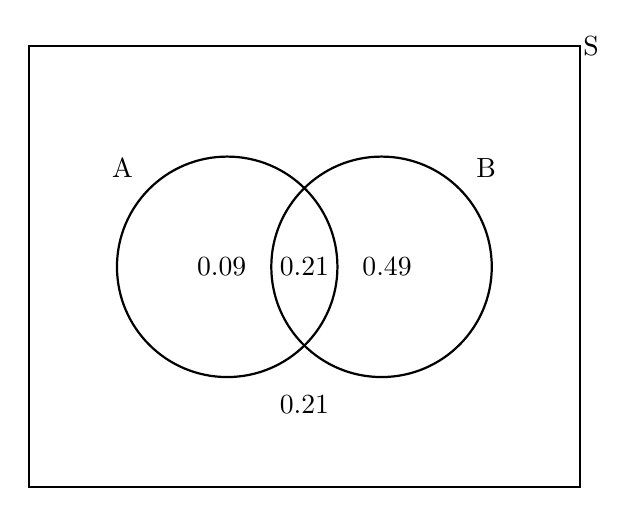
\begin{tikzpicture}[scale = 0.7]
  % Le rectangle
  \draw[thick] (-5,-4) rectangle (5,4);
  
  % Les cercles
  \draw[thick] (-1.4,0) circle (2);     % S
  \draw[thick] (1.4,0) circle (2);      % P
 
  
  % Les lettres
  \node at (-3.3,1.8) {A};
  \node at (3.3,1.8) {B};
  \node at (-1.5, 0) {0.09};
  \node at (0,0) {0.21};
  \node at (1.5, 0) {0.49};
  \node at (0, -2.5) {0.21};
  \node at (5.2, 4) {S};

  
\end{tikzpicture}
\end{center}

\end{frame}

\begin{frame}[t]{Exemple 6}

Il est possible que $A\perp B$, $A\perp C$ et $B\perp C$, mais
que $A,B,C$ ne
Soit pas indépendants. Par exemple

\begin{center}
    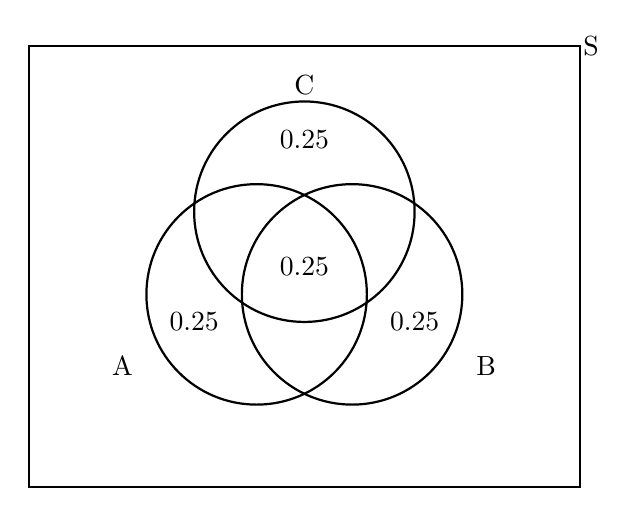
\begin{tikzpicture}[scale = 0.7]
  % Le rectangle
  \draw[thick] (-5,-4) rectangle (5,4);
  
  % Les cercles
  \draw[thick] (-0.866,-0.5) circle (2);     % S
  \draw[thick] (0.866,-0.5) circle (2);      % P
  \draw[thick] (0,1) circle (2);    % F
  
  % Les lettres
  \node at (-3.3,-1.8) {A};
  \node at (3.3,-1.8) {B};
  \node at (0,3.3) {C};
  \node at (-2,-1) {0.25};
  \node at (2,-1) {0.25};
  \node at (0,2.3) {0.25};
  \node at (0,0) {0.25};
  \node at (5.2, 4) {S};
\end{tikzpicture}
\end{center}

\end{frame}

%\section{Loi des probabilités totales, théorème de Bayes}

\subsection{Loi des probabilités totales}

\begin{frame}[t]{Partitionner l'espace échantillonal}

{\small Plusieurs problèmes de calcul de probabilités
 deviennent plus simples si on les divise en
 plusieurs morceaux. %À cette fin, nous voudrons  \alert{partitionner} l'espace échantillonnal.

 \begin{Boite}{Partition de l'espace échantillonnal}
  On dit que $B_1,B_2,\ldots,B_k$ forment une \alert{partition
  de $S$} si et seulement si
  \begin{enumerate}
   \item ils sont mutuellement exclusifs, i.e., $B_i\cap B_j=\emptyset,\ \forall i\neq j$\\

   \underline{et}
   \item leur union est $S$: $B_1\cup B_2\cup ...\cup B_k=S$.
  \end{enumerate}
 \end{Boite}
}
\end{frame}

\begin{frame}[t]{Exemple d'une partition de $S$}

\begin{center}
    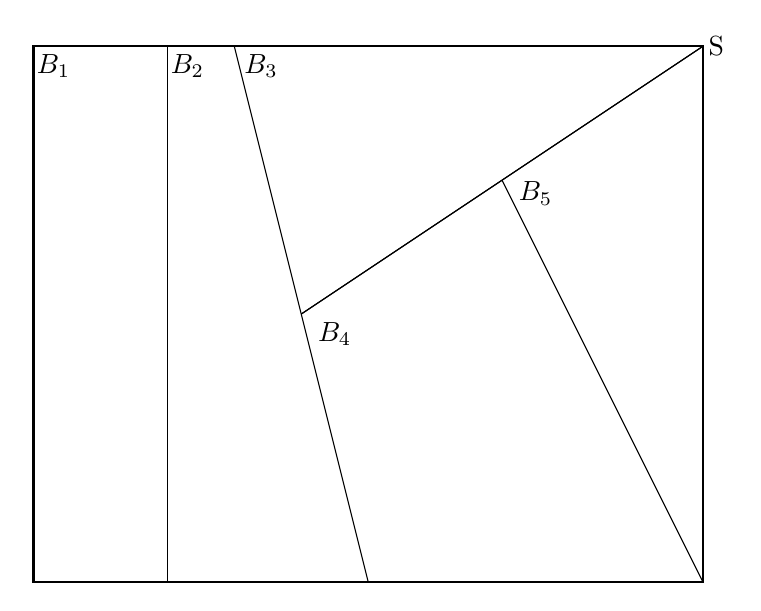
\begin{tikzpicture}[scale = 0.85]
  % Le rectangle
  \draw[thick] (-5,-4) rectangle (5,4);
  
  % Les cercles
  \draw (-3,4) -- (-3,-4);
  \draw (-2,4) -- (0,-4);
  \draw (-1,0) -- (5,4);
  \draw (-1,0) -- (5,4);
  \draw (2,2) -- (5,-4);
  
  
  % Les lettres
  \node at (-4.7,3.7) {$B_1$};
  \node at (-2.7,3.7) {$B_2$};
  \node at (-1.6,3.7) {$B_3$};
  \node at (-0.5,-0.3) {$B_4$};
  \node at (2.5,1.8) {$B_5$};
  \node at (5.2, 4) {S};

\end{tikzpicture}
\end{center}

\end{frame}


\begin{frame}[t]{Utilité de partitionner $S$}
 \begin{Boite}{Lemme}
  Si $B_1,\ldots,B_k$ forment une partition de $S$ et
  $A$ est un événement dans $S$, alors
  $$A=(A\cap B_1)\cup(A\cap B_2)\cup\cdots\cup(A\cap B_k).$$

  Puisque $(A\cap B_i)\cap(A\cap B_j)=\emptyset,\ \forall i\neq j$, on a que
  \begin{align*}
  P(A)&=P(A\cap B_1)+P(A\cap B_2)+\cdots+P(A\cap B_k)\\
  \alert {P(A)} &\alert{=\sum_{i=1}^kP(A\cap B_i)}.
  \end{align*}
 \end{Boite}
\end{frame}

\begin{frame}[t]{Exemple d'une partition de $S$}

\begin{center}
    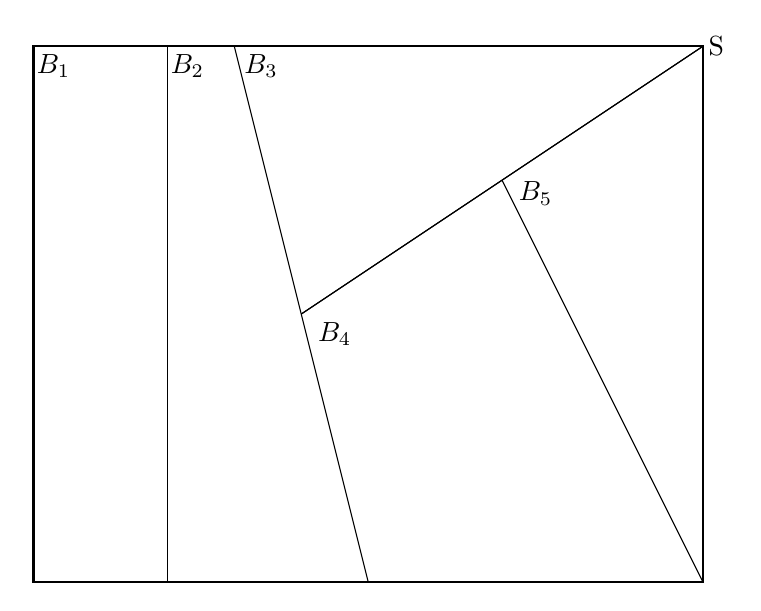
\begin{tikzpicture}[scale = 0.85]
  % Le rectangle
  \draw[thick] (-5,-4) rectangle (5,4);
  
  % Les cercles
  \draw (-3,4) -- (-3,-4);
  \draw (-2,4) -- (0,-4);
  \draw (-1,0) -- (5,4);
  \draw (-1,0) -- (5,4);
  \draw (2,2) -- (5,-4);
  
  
  % Les lettres
  \node at (-4.7,3.7) {$B_1$};
  \node at (-2.7,3.7) {$B_2$};
  \node at (-1.6,3.7) {$B_3$};
  \node at (-0.5,-0.3) {$B_4$};
  \node at (2.5,1.8) {$B_5$};
  \node at (5.2, 4) {S};

\end{tikzpicture}
\end{center}
\end{frame}

\begin{frame}[t]{Conditionner sur une partition pour trouver $P(A)$}
 \begin{Boite}{Théorème 1.8: Loi des probabilités totales}
  Soit $A$ un événement dans $S$ et $B_1,\ldots,B_k$ une partition
  de $S$. Alors
  $$\begin{array}{llccccc}
P(A)&=& P(A\cap B_1) &+&...&+&P(A\cap B_k)\\
&&&&&&\\
    &=&P(B_1)P(A|B_1)&+&...&+&P(B_k)P(A|B_k)\\
&&&&&&\\
    &=&\multicolumn{5}{l}{\sum\limits_{i=1}^k P(B_i)P(A|B_i)}\\
\end{array}
$$
 \end{Boite}


 \bigskip
 \underline{Cas particulier}: Comme $B$ et $\overline{B}$ forment une partition
 de $S$, on a $P(A)=P(A|B)P(B)+P(A|\overline{B})P(\overline{B})$.
\end{frame}
\begin{frame}[t]{Exemple 7}

{\small Un certain étudiant est à l'heure 75\% du temps. Quand il est à l'heure, il écoute le cours 90\% du temps. Quand il n'est pas à l'heure, il écoute 20\%
 du temps.

\begin{enumerate}\itemsep 2cm
\item[a)] Quelle est la probabilité qu'il ne soit pas à l'heure et qu'il n'écoute pas?
\end{enumerate}



}
\end{frame}
\begin{frame}[t]{Exemple 7 (suite)}

{\small
\begin{enumerate}\itemsep 2cm
\item[b)]  Quelle est la probabilité qu'il écoute?
\end{enumerate}


 \vspace{5 cm}
 %Il serait tellement plus simple de répondre à cette question  si on savait mon humeur ... $\Rightarrow$ On conditionne sur mon  humeur à l'aide de la loi des probabilités totales!!
}
\end{frame}

\begin{frame}[t]{Exemple 8}

{\footnotesize Un fabricant de dispositifs biomédicaux souhaite évaluer la performance à long terme de ses dispositifs afin d’orienter le choix des matériaux pour les prochaines générations de produits.
\begin{enumerate}[$\bullet$]
\item 50 \% sont fabriqués à partir du matériau A ;
\item 30\% sont fabriqués à partir du matériau B ;
\item 20\% sont fabriqués à partir de matériaux alternatifs.
\end{enumerate}

Les études de suivi clinique montrent que :
\begin{enumerate}[$\bullet$]
\item 90 \% des dispositifs fabriqués en matériau A demeurent fonctionnels sans intervention chirurgicale majeure pendant plus de 10 ans ;
\item cette proportion est de 80 \% pour les dispositifs en matériau B ;
\item elle est de 70 \% pour les implants fabriqués à partir de matériaux alternatifs.
\end{enumerate}





    
}
\end{frame}

\begin{frame}[t]{Exemple 8 (suite)}
Tracez un diagramme en arbre et un diagramme de Venn qui schématisent cette situation.
 \vspace{7cm}
\end{frame}

\begin{frame}[plain,t]%{Exemple 8(suite)}


\centerline{\LARGE\bf\alert{QUIZ !}}
Exemple 8: Quelle est la probabilité qu'un dispositif pris au hasard demeure fonctionnel sans intervention chirurgicale majeure pendant plus de 10 ans?

 \vspace{5.6cm}

\end{frame}

\subsection{Théorème de Bayes}

\begin{frame}[t]{Quand l'information est donnée «à l'envers» ...}
 Pour plusieurs problèmes, on donne l'information sous la forme $P(A|B_i)$,
 mais on nous demande de calculer $P(B_i|A)$.

 \begin{itemize}\itemsep 1cm
  \item Dans l'exemple 7, quelle est la probabilité que l'étudiant soit arrivé à l'heure sachant qu'il écoute?
  \item Dans l'exemple 8, si un dispositif est demeuré fonctionnel moins de 10 ans, quelle est la probabilité qu'il soit fait de matériau de type B?
 \end{itemize}
\end{frame}

\begin{frame}[t]%{Théorème de Bayes}
 \begin{Boite}{Théorème de Bayes}
  Soit $A$ un événement dans $S$ et $B_1,\ldots,B_k$, une partition
  de $S$. Alors
  $$P(B_j|A)=\frac{P(A|B_j)P(B_j)}{\sum_{i=1}^kP(A|B_i)P(B_i)},\ \ \forall j=1,\ldots,k.$$
 \end{Boite}

 %\underline{Preuve}:
\end{frame}

\begin{frame}[t]{Exemple 7 (suite)}

Quelle est la probabilité que l'étudiant soit arrivé à l'heure sachant qu'il écoute?

\end{frame}


\begin{frame}[plain,t]%{Exemple 8(suite)}


\centerline{\LARGE\bf\alert{QUIZ !}}

  \vspace{2mm}
  Un dispositif a nécessité une intervention chirurgicale avant 10 ans. Quelle est la probabilité que ce dispositif soit fait de matériau
  de type B?
 \vspace{5cm}

\end{frame}

\begin{frame}[t]{Réponses aux exemples}

\footnotesize
\begin{enumerate}
  \item ${\cal{E}}_1$:  $ {{S}}_1=\{1,2,3,4,5,6\}$;  ${\cal{E}}_2$: $  {{S}}_2=\{R\spadesuit,R\heartsuit,R\diamondsuit,R\clubsuit\}$;\\${\cal{E}}_3$: $ {{S}}_3=\{0,1,2,\ldots\}$;${\cal{E}}_4$: $ {{S}}_4=\{x:x\ge0\}$.
  \item $P(\overline B)= 0,80,\; P(A\cap B)=0,02$
  \item $P(\overline F)=0,45,\;P(F\cap S)=ND, \; P(F\cap S)=0,45,\;P(\overline F\cap S)=0,30, \; P(\overline F\cap S\cap P)=ND,\;P(S\cup F)=0,85,\;P(F|S)=0,6,\;P(P|F)=7/11$
  \item $P(D|A)=1/7,\; P(B|D)=3/5$
  \item Oui
  \item $P(A\cap B\cap C)\ne P(A)P(B)P(C)$
  \item $P(\overline E\cap \overline H)=0,20\; P(E)=0,725, P(H|E)\approx 0,931$
  \item S'inspirer de l'exemple 7
 \end{enumerate}
\end{frame}

\end{document}